%%% Local Variables:
%%% mode: latex
%%% TeX-master: "../report"
%%% End:

% Detailed description of goals
%% Brief recap of WHAT we want to solve
%% Details of HOW we gon do dat

\subsection{Stack Management}
%% Basic
%% Stack vs. Register
%%% (see background)
%% Threaded
%% Stack element
%%% Type
%% Manipulation (instr)

Stack is an abstract data type, fundamental in the fields of algorithms and
computer science. It is a very simple model only requiring two essential
functions, {\it push} and {\it pop}, as visualized in
figure~\ref{fig:stack}. Push adds an element to a stack of elements, while pop
removes the top most element. As an analogy, imagine a spring loaded tray of
clean dishes where one can only take from the top. When adding a new dish it
becomes the new top-most dish in the stack. This sequence of adding and taking
from a collection of element is called Last In, First Out (LIFO).
\begin{figure}[h]
  \centering
  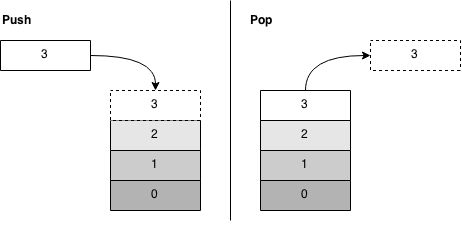
\includegraphics[scale=0.6]{images/stack.png}
  \caption{Stack push and pop operations}
  \label{fig:stack}
\end{figure}

% The stack was first introduced in 1946 by Alan Turing, while he was working on
% the Automatic Computing Engine (ACE)~\footnote{Automatic Computing Engine (ACE):
% \url{http://en.wikipedia.org/wiki/Automatic_Computing_Engine}} at the National
% Physical Laboratory (NPL)~\footnote{National Physical Laboratory:
% \url{http://en.wikipedia.org/wiki/National_Physical_Laboratory_(United_Kingdom)}}
% in the UK:
% \begin{quote}
%   [Alan Turing] outlined a method for leaving one line of work being carried out
%   on the computer, calling up a subsidiary line, and then returing to the first
%   line when finished with the subsidiary line. He called the calling up and
%   returning routines BURY and UNBURY.~(\textcite[82]{newton})
% \end{quote}
% Here, BURY and UNBURY are synonymous with push and pop.

% @book{newton,
% author    = "David E. Newton",
% year      = 2003,
% title     = "Alan Turing : a study in light and shadow",
% publisher = "[Philadelphia]: Xlibris",
% ISBN      = 9781401090791
% }

Although, essentially, one cannot take the second element from top without first
removing the top most element, the model can easily be modified to support such
operations. For instance, a common stack operation is {\it peek}, which reads
the value of the top element without actually removing it. This can easily be
done by popping, storing the value and pushing it back to the stack. Other
operations can be implemented in a similar fashion.

\subsubsection{Stack vs. Register Machine}
Machines can both implement the stack model physically and virtually, but as we
are designing an abstract machine, we will only discuss the virtual
aspect. Regardless, such a machine is commonly called a \term{stack machine}.

The most common notation in arithmetic formulas and statements are the infix
notation, where the operator is written between its operands: $1 + 2$. One can
express the same statement with prefix notation, also called \term{Polish
  notation}: $+\ 1\ 2$. When programming stack machines, one uses what is called
the \term{reverse Polish notation}, which is in fact postfix notation:
$1\ 2\ +$. By using this notation, one can easily convert this into stack
operations, where $1\ 2\ +$ becomes:
\begin{stackops}
  \op{push 1}{1}
  \op{push 2}{2,\ 1}
  \op{add}{3}
\end{stackops}

Here the {\tt add} operation pops two elements, adds them together and pushes
the result back onto the stack.

As briefly discussed in the~\nameref{sec:background} section, a register machine
TODO

\subsubsection{Threading}
Big chip manufacturers like Intel, have always been under big pressure to
deliver ever faster processors, year after year. For around the last decade, the
technological development of processors has been focused adding cores rather
than increasing the clock speed, which already started to stagnate around
2004~\cite{sutter}. With multiple processors, or popularly called a multi-core
processor, processes may actually run in parallel, i.e. running at the same
time, rather than just concurrently where multiple processes actually share the
same processor.

A thread is typically the smallest unit of executable instructions by a
processor. A process being run by an operating system therefor had one thread
which the operating systems scheduler delegated CPU time to. With multi-core
processors, the notion of a single process having multiple threads arose, making
it possible for a process to compute several things concurrently (not
necessarily in parallel). This is known as multi-threading, and is commonly
supported by most modern operating systems.

Although multi-threading is a very interesting feature, it also raises a lot of
challenges when designing machines. Different threads cannot directly read and
write to the same, without taking data races into account, which is a common
mistake when writing multi-threaded programs. If multiple threads are accessing
the same memory, it can change at any time and therefor cannot be TODO

As with our stack machine, each thread has to have its own state, including its
own stack. In other words, all stacks are private and cannot be shared across
threads. This can though be simulated using heap object which are referenced
from multiple threads' stack.

TODO: tasks and transactions
% Multiple executables may execute simultaneously.
% Task and transaction semantics is supported. A transaction is considered
% executed by the thread starting it. A spawned task is independent of the spawn-
% ing thread and may be executed by the spawning thread or some other thread.
% However, tasks will not migrate between threads so the thread which started
% execution of a task will also complete the task.

% Tasks do not share stacks with the spawning thread, spawning task, or any
% other task. Implementations may, however, execute tasks using the stack of the
% executing thread. The executed task is not allowed to access any stack space
% beyond its initial set of stack elements. The implementation must throw an
% exception if any such offending access is attempted.

\subsubsection{Stack Organization}
% All stacks will initially have a single activation frame

The stacks will not be limited in size, as the compilers will be able to
implement stacks as heap object which can grow dynamically. Through out this
report, we will say that the stacks \term{grows downwards}. This is because
physically, the top most element of the stack is located at a low address in the
host computers memory. Therefor, as more elements are pushed to the stack, they
will get higher addresses, making the stack grow downwards in memory.

A stack element will consist of some type information and a reference to its
content, or data. The type information will include its declared type, but also
an actual type. For statically typed languages, these will most likely (TODO: ?)
be the same. For dynamic languages this is required to hold track of an
element's type, as its allowed to assign a value type an element, which was
originally declared with an other type.

\subsubsection{Stack Manipulation}
As mentioned above, there will we instructions for doing simple stack
manipulations, for instance {\tt push} and {\tt pop}. As we will see later,
these two instructions alone will be very limiting, and make the job of writing
a compiler very tedious. Therefor, we will need more instructions, making more
complex manipulations more convenient.

Later, when we will describe the execution model of the machine, we will see
that instructions for pushing an popping elements further up the stack. For
instance, if we want to access the arguments given to a subroutine, they will be
located up the stack. The compiler will therefor need an effective method of
duplicating that element onto the top of the stack, making is accessible for
further computation. Also it will need to push an element to a specific position
up the stack, effectively returning a value to the caller.

Such versions of the push and pop operations will take an displacement argument,
saying how many places up the stack it is to push to or pop from. To make this
as convenient as possible, the displacement will be from the top of the stack,
meaning displacement 0 will be the top of the stack. Exception handling will
have to be utilized when using a displacement which is not allowed, for instance
outside the stack or its own scope.

Lets call these two instructions {\tt pushElement} and {\tt popElement}. Unlike
{\tt push}, which adds a new element to the stack, we have chosen that {\tt
  pushElement} will overwrite the element at the given displacement. This is
more convenient as this does not change the displacement of the following
elements, though it requires some planning, as there will have to be an element
on the stack with the purpose of being overwritten.

Also, unlike our previous stack example, the {\tt push} instruction, or rather
the {\tt pushElement} instruction, will not take a value as an argument. Rather
it will take the top element and push it to the place of the given displacement
argument. There will be separate instructions for adding new elements onto the
stack, for instance {\tt pushConstant}.

Here we can see some simple operations using the {\tt pushElement} and {\tt
  popElement} operations.
\begin{stackops}
  \op{-}{3,\ 1,\ 1}
  \op{pushElement 0}{3,\ 1,\ 3}
\end{stackops}



% Examples of how to map things to our model ()
%% Classes
%% Inheritance
%% HoF
%% Polymorphism

% Type system
%% Representation (DWARF)
%% Typed instructions
%% Run-time type checking
%% Dynamic types
%%% !!!

% Executable format
%% ELF
%%% It's tried-and-true
%%% Everybody else uses it so we can port stuff easier

% Object model
%% Virtual tables
%% Hash maps
%%% How is it different from using vtables
%%% The efficiency of them
%% Dynamic dispatches

% Threading
%% Tasks and transactions
%%% Shared stack elements
%% ?!

% Closures

% Memory management
%% Garbage collection

% ISA
%% Highlight the most important instructions, explain how they facilitate the above
